\documentclass[border=8pt]{standalone}
\usepackage{amsmath}
\usepackage{amssymb}
\usepackage{xcolor}
\usepackage{tikz}
\usetikzlibrary{arrows.meta,calc,decorations.pathreplacing,patterns,shapes.geometric,positioning,shadings,plotmarks}

\definecolor{bgdark}{HTML}{0B1A2A}
\definecolor{horizon}{HTML}{F2D27A}
\definecolor{accent}{HTML}{F4A437}
\definecolor{lightgrey}{HTML}{D8D8D8}

\begin{document}
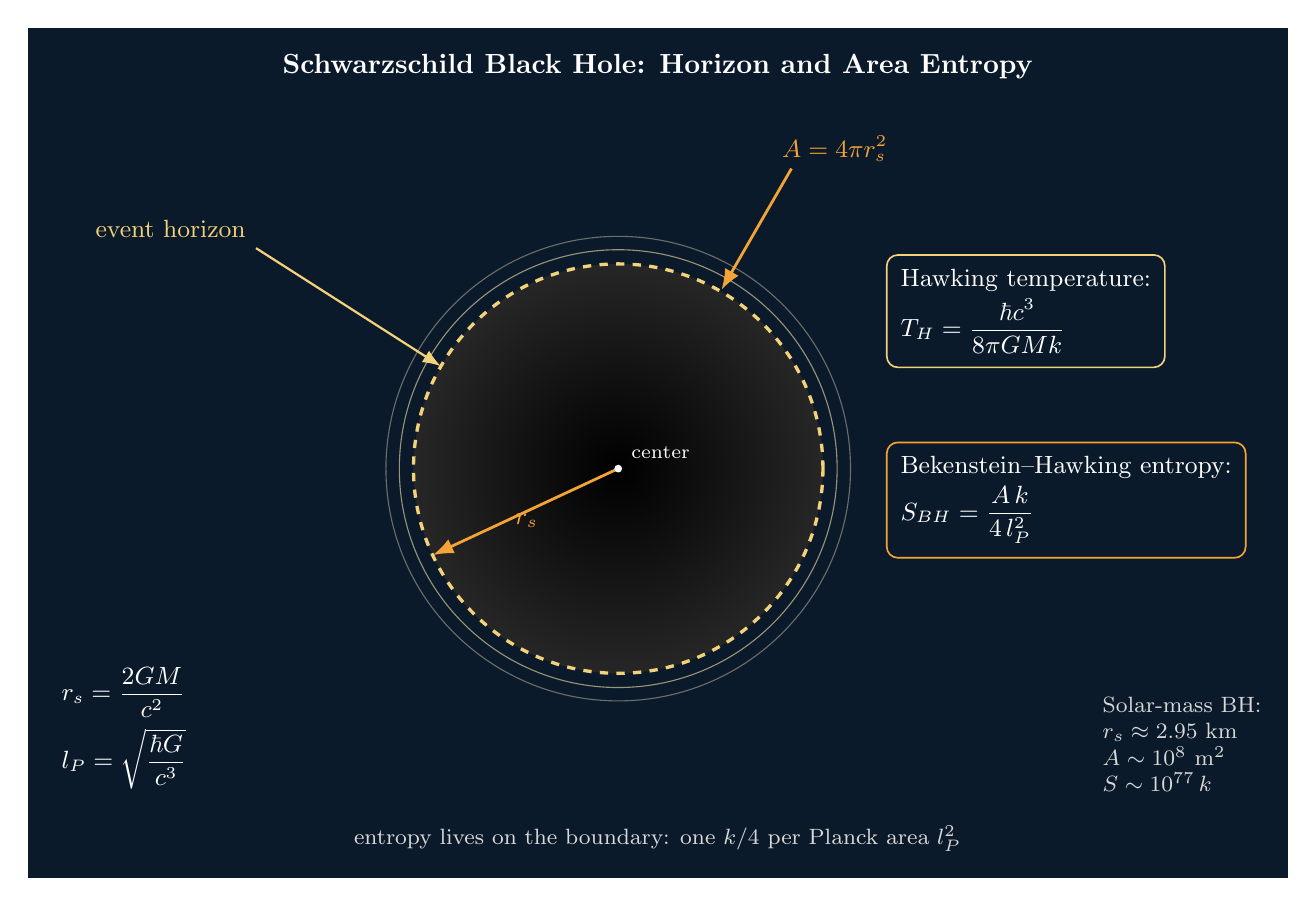
\begin{tikzpicture}[>=Latex,thick]

% Dark background
\fill[bgdark] (-7.5,-5.2) rectangle (8.5,5.6);

% Title
\node[white, font=\bfseries] at (0.5, 5.1)
  {Schwarzschild Black Hole: Horizon and Area Entropy};

% Center of black hole
\coordinate (C) at (0,0);

% Black hole sphere (filled black with subtle radial shading toward edge)
\shade[ball color=black!95, inner color=black, outer color=black!85]
  (C) circle (2.6);

% Event horizon: dashed yellow circle, slightly larger than the BH body
\draw[horizon, dashed, line width=1.2pt] (C) circle (2.6);

% Faint outer halo to suggest horizon glow
\draw[horizon!60, line width=0.4pt, opacity=0.6] (C) circle (2.78);
\draw[horizon!40, line width=0.4pt, opacity=0.4] (C) circle (2.95);

% r_s arrow: from center along radial direction (angle ~ 200 deg, into BH lower-left)
\coordinate (Rend) at ({2.6*cos(205)},{2.6*sin(205)});
\draw[accent, line width=1.0pt, ->] (C) -- (Rend);
\node[accent, font=\small] at ({1.45*cos(205)+0.15},{1.45*sin(205)-0.05})
  {$r_s$};

% Center dot
\fill[white] (C) circle (1.4pt);
\node[white, font=\scriptsize, above right=0pt and 1pt of C] {center};

% Area arrow: from outside pointing to horizon (angle ~ 60 deg, upper-right)
\coordinate (Aout) at ({4.4*cos(60)},{4.4*sin(60)});
\coordinate (Ain)  at ({2.62*cos(60)},{2.62*sin(60)});
\draw[accent, line width=1.0pt, ->] (Aout) -- (Ain);
\node[accent, font=\small] at ({4.7*cos(60)+0.4},{4.4*sin(60)+0.25})
  {$A = 4\pi r_s^{2}$};

% Label "event horizon" pointing at the dashed circle (upper-left)
\coordinate (HzL) at ({-4.6},{2.8});
\coordinate (HzP) at ({2.6*cos(150)},{2.6*sin(150)});
\draw[horizon, line width=0.8pt, ->] (HzL) -- (HzP);
\node[horizon, font=\small, anchor=south east] at (HzL)
  {event horizon};

% Schwarzschild radius equation (lower-left)
\node[white, font=\small, align=left, anchor=west] at (-7.2, -3.3)
  {$r_s = \dfrac{2GM}{c^{2}}$ \\[3pt]
   $l_P = \sqrt{\dfrac{\hbar G}{c^{3}}}$};

% Hawking temperature box (right side)
\node[draw=horizon, line width=0.6pt, rounded corners,
      fill=bgdark, text=white, font=\small, align=left,
      anchor=west, inner sep=5pt]
  at (3.4, 2.0)
  {Hawking temperature: \\[2pt]
   $\displaystyle T_H = \frac{\hbar c^{3}}{8\pi GMk}$};

% Bekenstein-Hawking entropy box (right side, lower)
\node[draw=accent, line width=0.6pt, rounded corners,
      fill=bgdark, text=white, font=\small, align=left,
      anchor=west, inner sep=5pt]
  at (3.4, -0.4)
  {Bekenstein--Hawking entropy: \\[2pt]
   $\displaystyle S_{BH} = \frac{A\,k}{4\, l_P^{2}}$};

% Solar-mass numbers (lower-right)
\node[lightgrey, font=\footnotesize, align=left, anchor=east] at (8.3, -3.5)
  {Solar-mass BH: \\
   $r_s \approx 2.95~\mathrm{km}$ \\
   $A \sim 10^{8}~\mathrm{m}^{2}$ \\
   $S \sim 10^{77}\,k$};

% Caption-line below
\node[lightgrey, font=\footnotesize] at (0.5, -4.7)
  {entropy lives on the boundary: one $k/4$ per Planck area $l_P^{2}$};

\end{tikzpicture}
\end{document}
